\documentclass{UoYCSproject}

\usepackage{fullpage}
\usepackage{amsmath}
\usepackage{color}
\usepackage{graphicx}
\usepackage{tikz}
\usetikzlibrary{positioning,shapes.geometric}

\title{Towards a Building Modelling Framework: Heuristic-EZ}
\MEng{}
\author{Martin Higgs}
\date{\today}
\supervisor{Iain Bate}
\wordcount{\textcolor{red}{TODO}}

\abstract{
	Estimate (for BSc!):
	\begin{itemize}
		\item Abstract, ethics statement, etc. - 500 \textcolor{red}{(0)}
		\item Introduction - 1,000 \textcolor{green}{(881)}
		\item Literature review - 3,000 \textcolor{green}{(4,104)}
		\item Problem description/analysis - 1,500 \textcolor{green}{(1,350)}
		\item Design and implementation - 2,500 \textcolor{green}{(3,707)}
		\item Results and evaluation - 2,500 \textcolor{red}{(0)}
		\item Conclusion - 1,000 \textcolor{red}{(0)}
	\end{itemize}
	\textcolor{red}{Total word count: 10,631 (including notes)}
}

\acknowledgements{Thanks to Iain Bate in his role of supervisor, without whom's support and guidance this project may never have seen success. Also thanks to \citeauthor{torres2014ujiindoorloc} for their eager responses and wide data set enabling great future insight and broad analysis.}

\begin{document}
	
	\maketitle
	
	\chapter{Introduction}
    \label{chap:intro}
    
        Modern buildings can be technological marvels with beautifully designed spaces to get the maximum amount of light to every corner. Navigating these spaces however can be another beast entirely with different layouts and separations across multiple floors and only the occasional abstractly designed map stating ``You are here''. With the prevalence of sensor-packed smart-phones, outdoors your simplest recompense might be to ask the mighty Google (or your preferred mapping software) and within seconds you can be told exactly which muddy field you are trudging through along with a crisp satellite image of the area. Indoors, these positioning technologies rapidly lose their accuracy, either giving up entirely or if not declaring your location to be somewhere within the next 5 buildings.
        
        This rapid loss of accuracy is due to the loss of visibility to the small number of landmarks from which your position is determined. Contrarily, one of the currently most effective ways to localise yourself in a strange place is to ask a fellow wanderer who might use their experiences to give you directions based on numerous smaller landmarks within the space (such as a shop or fountain). In a similar manner, might it not be more effective to use our sensor-enabled devices to build a shared picture of the space using machine-identifiable landmarks (like magnetometry or radio data)?
        
        This is the aim of this project: to create a framework wherein researchers and real-world deployments alike can collect data from a large number of devices traversing their space and use it to create a model that users can locate themselves in. Though it should be noted that most often machine-identifiable landmarks and those used by people do not overlap. As such investigations will also be made into how machine learning might be able to translate these data points into other characteristics of the space, like a human-readable floor map. 
        
        The uses and sources of information that could be pooled for this purpose are virtually unbounded from timetabling schedules to security check-ins to emergency situation planners, so a flexible, verifiable implementation could be extensively useful. But of course, not all information is complete, freely available, accurate or even relevant to every application. Creating this framework will enable collaboration across teams working on multiple techniques by providing them with an array of common components to evaluate against.
        
        As such this project will look into:
        \begin{itemize}
        	\item Potential crowd-sourced data gathering techniques, both pre-existing and theoretical improvements
        	\item Data sources used in various indoor positioning systems
        	\item Machine learning techniques for turning this data into a functional model
        	\item Creating or acquiring freely available data sets to enable common evaluation
        	\item Translating models and data into a human readable format
        \end{itemize}
        
        While it would be foolish to assume that research already exists on or that this singular project could accomplish all of these goals in a single blow, it might be pessimistic to assume that none of these goals are already sufficiently covered in the real world. As such this project will assess the related literature and make the best possible start towards a unified building analytical framework. Ideally this project will produce a piece of software collecting or modelling data with an associated example data set and a set of experimental results for comparison against future works.
        
        This is of course not without anticipated challenges. For one, when crowd-sourcing, how might the user be provided with the utmost respect, both for their privacy and such as not to impede their daily life, while still aiming to collect a diverse and representative data set? When modelling data, how might the system deal with noisy or unreliable data and then make comparisons against more credible sources of information for correctness? And finally, when translating this all into more useful or human readable data, what actually makes each model good?
        
        Before attempting to answer these questions, the ethical connotations of this study should also be considered. Given the unknown applicability of data for building these models, it would make sense to build a crowd-sourcing application that can target as wide a user-base as possible for as many types of data as possible. Thereby, if the techniques for gathering data are so subtle that the user might never notice an installation of an application of this nature, there is the possibility that it could be deployed maliciously. Further, should the modelling techniques prove successful at generating human-readable maps from the user's data, given enough time theoretically any space could be mapped, with or without the owner's consent. These concerns however are generally mitigated by modern mobile operating systems allowing user's fine-grain control over application's access to data and secure locations often banning the use of foreign mobile technology entirely.
        
        With all of these points in mind, this report will be broken down into the following chapters, documenting the project's progression. Chapter \ref{chap:related} will cover a review of the existing work surrounding the project's goals while chapter \ref{chap:problem} will then attempt to identify the most significant contribution possible in line with the those goals while maintaining a manageable scope. Chapter \ref{chap:method} will document the process of creating the initial components of the framework this project aims to create and chapter \ref{chap:eval} will attempt to evaluate it against other documented techniques. Finally, chapter \ref{chap:conclusion} will provide an overview of the entire experience, including future work and the non-functional attributes described previously.
        
	\chapter{Related Work}
    \label{chap:related}
	
		This chapter conducts a review of various works surrounding the project's goals. First it will address the motivations and support the relevance of this study (Section \ref{sec:motivations}). Concluding that it will provide coverage of the constituent parts relevant to the work on crowd-sourcing the data to be used, indoor positioning systems for creating a location map of the data and finally the automated generation of floor plans for analysis of the building in sections \ref{sec:crowd}, \ref{sec:ips} and \ref{sec:floorplans} respectively.
        
        \section{Motivations}
        \label{sec:motivations}
        
            Modelling a building by various methods for automation and analysis can provide a multitude of benefits through better understanding of its use from emergency situation handling to day-to-day improvements. For example \citet{gao2009self} provide an extremely simple method for intelligently setting the on/off times for central heating, increasing energy efficiency while minimising user discomfort. The method is built around using smart-home sensors (such as reed switches on doors or motion detectors) to determine the latest leaving (to work) and earliest entrance (from work) times and incorporating these with a user-specified amount of ``miss time'' when the house is occupied but the house is not already warm. As the technique is flexible with regards to user-defined worst-case performance and the number of users under observation, with the prevalence of WiFi enabled personal devices, it could easily be adapted to monitor user's devices leaving / moving around the WLAN and scaled to larger buildings with finer grain control over their heating.
            
            By giving the system control over a user's environment however, it enters into a category of ``physical computing systems'' as identified by \citet{stankovic2005opportunities}. While this is a very simple definition of any system that can take in data through some collection of sensors (e.g. a Wireless Sensor Network) and act upon that data through some actuators, one must be aware of the responsibility placed upon the system. Most of the concerns raised are context sensitive, but when designing such a technique it can help to consider these situations in order to identify its limitations. Examples of such systems might include the use of WiFi signal scattering to detect and alert of falls in vulnerable homes \citep{han2014wifall}, provision of city-wide traffic management through a wireless network of cameras and signals \citep{LATraffic} or asset and personnel tracking across a wirelessly networked environment \citep{Ekahau}.
		
            The idea of leveraging wireless networks and the multitude of sensor-enabled devices that occupy them however has been around for quite some time. Recently \citet{torres2014ujiindoorloc} identified the specific trend for using such devices to provide Indoor Positioning / Localisation Systems (IPS), but no definitive way of comparing such techniques existed and so they created the UJIIndoorLoc database. This data set will be expanded upon later, but for now it serves to show the collaborative effort going into solving the problem of indoor localisation.
                
        \section{Crowd-sourcing Data}
        \label{sec:crowd}
        
            With the sheer variety of sensors available in modern personal devices carried by people of all backgrounds almost everywhere, sourcing as much data as possible would seem to be relatively easy. However, when using this technique the data collection must always attempt to be as un-invasive as possible. 
            
            An early endeavour into this field was CenceMe, a classification program designed to relay information about the user to their friends through Facebook \citep{miluzzo2008sensing}. The program ran on the Nokia N95 passively collecting data whenever the phone was interacted with (i.e. through button presses) which were then translated through a simple set of classifications into facts to pass on to the server for processing to Facebook. Collected data included GPS location, microphone noise, accelerometer data, Bluetooth device visibility and random pictures for determining where the user was, whether they were having a conversation, their activity level, who they were with and verification purposes respectively. Initially, the user needed to define people and places significant to them for the classifier to recognise but after this, CenceMe only needed prompt the user for input if it recognised a place the user visited frequently, in order for them to add it as a location to notify their friends about.
            
            Concerns raised during this study included those of privacy, portability, ease of development and power usage, most of which have been addressed by advances in mobile operating systems such as Android and iOS. When developing for the N95 the CenceMe team reported very limiting factors designing their framework including low memory, computational power and general programmability, all of which are not of concern today with multi-core, multi-gigabyte RAM devices running almost complete editions of Java with expansive APIs.
            
            However, with increased capability comes increased potential load on the device's power supply (high-speed cellular internet access and HD video processing are particular culprits), limiting its availability; as such manufacturers, OS providers and researchers alike are continually looking into power saving methods. One such team of researchers looked into a technique they called ``Piggyback Crowd-Sensing'' \citep{lane2013piggyback}. This technique centres around the multi-functional abilities of the devices carried today, for example the GPS sensor may be used for geo-tagging pictures, navigation or social media posts. This provides a crowd-sensing application with a variety of opportunities to utilise the GPS without powering up and winding down the sensor specifically to take measurements; `piggybacking' off of another applications sensor usage. 
            
            The problem with this technique arises with the need to narrow down the window of when / where sensor readings are taken as user application usage can be quite sporadic. The research team then complemented this method with a ``Sensing Decision Engine'' (prediction algorithm) that gathers data on which sensor-using apps were launched in which time windows (6 hour slots of each day), whether it was the weekend or a weekday when it was called up and which square kilometre it was used in. Based on these data, the algorithm is then able to predict whether a sensor is likely to be used in the current situation and so whether it should wait for the sensor to come into use or to power it up on its own. This technique as a whole was shown to save up to 90\% of the energy required to perform crowd-sensing for a small cost to the accuracy of readings. Successes in approaches like these have lead to adoptions at an operating system level, such as the Android ``Sensor Batching'' approach \citep{AndroidSenseBatch}.
            
            The location required for this sensing decision engine is intentionally broad as very low accuracy location estimates can be made through triangulation from nearby cellular signal towers. Gathered data however can require a much finer grain location estimate to associate with in order to make it meaningful.
                
        \section{Indoor Positioning Systems (IPS)}
        \label{sec:ips}
        
            Outdoor positioning sensors are commonplace in most devices today with GPS being the dominant technique as a device can calculate its absolute position using only the visible satellites for trilateration. Indoor positioning however often requires a much finer level of precision and with GPS being largely invisible from indoors the problem is widely regarded as being unsolved such to the point that competitions are being regularly held to encourage new techniques \citep{MSLOCComp}. These can be split into  the infrastructured and infrastructureless categories where the former requires deployment of additional equipment around the environment (such as motion sensors or microphones) and the latter should not with the sole exception being the assumed existence of Wireless Access Points (APs).
            
            As a fundamental component of analysing what rooms are in use when is knowing where users are at a given time, this section will cover a variety of IPS techniques in detail. As such each technique will be judged by its pre-deployment effort (cost of extra infrastructure, measurement taking, computational cost etc.), level of prior knowledge required of the building and on-line (active) location accuracy.
            
            \subsection{Early Techniques}
            \label{sec:early}
            
                One of the earliest infrastructured approaches was the Active Badge Location System wherein personnel badges were equipped with infrared emitters sending uniquely identifying signals to be picked up by detectors set up in every room \citep{want1992active}. While the set-up proved extensible (up to 128 badges monitored at once with low conflict rate) and flexible (more sensors can be added / moved with the building) with cheap sensors and badges it still required detectors being wired into every room and as such could only provide room-level accuracy at best and only a vague idea of where each person had been in areas not covered by detectors (such as corridors). 
            
                The team also appears to cite ``radio signals that can penetrate the partitions found in office buildings'' as a negative effect as their technique utilises proximity as a binary indicator of where a person is. However, while the paper may have served as an inspiration to create proximity-based positioning techniques, many more modern methods have decided to use the radios in Wireless APs as a single AP can cover a much larger space than an IR detector. This raises additional challenges though in dealing with how radio signals propagate, as the strength of a radio signal can be mangled by the distance it's travelled,  the materials it's passed through (be it air, wood, jeans or people) and by waves themselves (electromagnetic waves can cause destructive and constructive interference on their own frequency, be they reflected or just transmitted from another source)! Given all of these problems \citet{whitehouse2007practical} evaluated the use of received Radio Signal Strength Indicators (RSSI) as a sole measure to judge distance. Their results confirmed that even in ideal outdoor situations with few obstructions ``small differences in vegetation such as the height of grass can have large effects on RSSI'' and ``Experiments in an indoor environment revealed no discernible pattern in RSSI, even in a large room with no walls and at the very lowest transmission power.''.
            
                Despite this potential for wildly fluctuating RSSI based on the environment \citet{bahl2000radar} were able to create a mathematical model for the RSSI based on the floor plan of the building in question; RADAR, one of the first infrastructureless IPS techniques. RADAR is built around their Wall Attenuation Factor (WAF) model:
            
                \begin{equation} \label{eq:WAF}
                    P(d) = P(d_0) - 10nlog\left(\frac{d}{d_0}\right) - \left\lbrace 
                        \begin{matrix}
                            nW * WAF & nW < C \\
                            C * WAF  & nW \geq C \\
                        \end{matrix}
                    \right.
                \end{equation}
            
                This model is a simple combination of the standard signal path loss model and a linear drop in power for each wall that the signal travels through. To break it down, $P(d)$ is the expected RSSI (in $dBm$) at distance $d$, where $d_0$ is a distance of $0$m or the access point's `Transmit Power'. This signal travelling through the air then decays logarithmically according to an unknown but fixed rate $n$. Finally a fixed amount of power ($WAF$) is lost for each wall ($nW$) up to a pre-determined cap ($C$) beyond which any extra walls make no difference as the signal is pretty much unidentifiable anyway. This model is then applied to approximate the RSSI of every access point at every position in the building (using the floor plan as a guide) the create an RSSI map of the building in question. Location is then a relatively simple task of matching up the user's visible RSSI from each access point and matching them to the closest approximate location. This technique was created to as an alternative to taking `empirical' measurements throughout the building to create the map by hand and while it is not as strong as taking empirical measurements (roughly 30\% increase in median error) it saves a significant amount of effort for such a simple model.
                
                \begin{figure}[h]
                    \label{fig:m2}
                    \caption{Model $M_2$ from \citet{madigan2005bayesian}.}
                    \centering
                        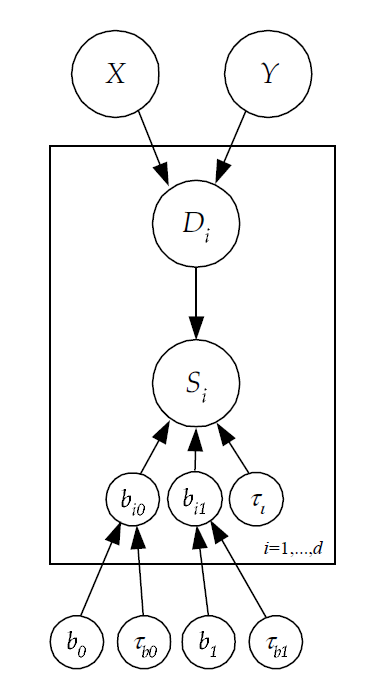
\includegraphics[width=0.3\textwidth]{Model_M2.png}
                \end{figure}
                
                \citet{madigan2005bayesian} instead utilised a graphical model to embody the relationship between position and RSSI (Figure \ref{fig:m2}). In their Bayesian Network, for each access point $i$ the distance $D_i$, transmit power $b_{i0}$, path loss rate $b_{i1}$ and noise $\tau_i$ are all conditionally dependant given the RSSI observed $S_i$. This signifies that given a set of these variables, the model can infer the most likely values for any connected values in the graph (for example, training data would give the X and Y co-ordinates and the signal strength, which can be used to infer all other variables given the graph's complete connected nature). Then during the on-line positioning phase, the user's most likely position is inferred from the AP variables established during the training phase and the observed RSSI values. Using this model they are able to estimate position assuming only the degradation of RSSI is roughly logarithmic and that all access points have similar behaviours ($b_0$ and $b_1$ are the global variables around which each specific access point's values are estimated). This method does require training data in order to calculate the maximum likelihood access point parameters, but with a very small number of training samples (around 20) and no other knowledge of the building they show that the model is able to estimate the user location with a \textasciitilde50\% increase in median error compared to RADAR.
                
                While providing insights into the area under observation with little prior knowledge, these techniques are 'one-shot': a model is built from known values and then followed permanently thereafter. However, should the space be modified at any point after the model is created, the solution would effectively need re-deploying to continue providing accurate estimates.
            
            \subsection{Adaptive Indoor Positioning Systems}
            \label{sec:adaptive}
            
                All of the previous techniques discussed have had two very distinct phases: off-line and on-line. During the off-line training phase, data is gathered with ground truths (guaranteed values such as user verified location) or models are calculated and then in the on-line positioning phase the observed RSSI values are then used in the models to determine the user's most likely location. This section however will explore techniques that can improve gradually over time as more users traverse the space.
                
                Techniques covered to this point rely on electromagnetic waves and the detection thereof to paint a picture of the user's current location, however \citet{wang2012no} combined dead-reckoning (estimating relative location by tracking movement from a known point) and a broader range of sensors than most other techniques to estimate location. Traditional dead-reckoning is known to be relatively accurate at first, but random errors gradually accumulate and the estimation can become wildly inaccurate the further travelled from the starting point. This technique however relies on organically generated `landmarks' to help reset the accuracy of a user's current position as frequently as possible (Figure \ref{fig:dead}). These landmarks can range from elevators detected by accelerometer spikes to metallic areas detected by the magnetometer, each uniquely identified by the RSSI values surrounding the area. As the mean of the error generated by dead-reckoning is theoretically $0$, a landmark can be placed at the average location of all positions it has been identified at making exact positioning when the landmark is detected possible. While accurate to a reported 1.2m with no prior knowledge of the space and no deployment necessary, this positioning method must be permanently active from each landmark or the user will be unable to locate themselves. Also, even with techniques identified to only use the most effective landmarks this would still put a relatively heavy weight on the user's power supply through its always-on nature and the variety of sensors required compared to conventional RSSI measurement.
                
                \begin{figure}[h]
                    \label{fig:dead}
                    \caption{Dead-reckoning accuracy found through experimentation by \citet{wang2012no}.}
                    \centering
                        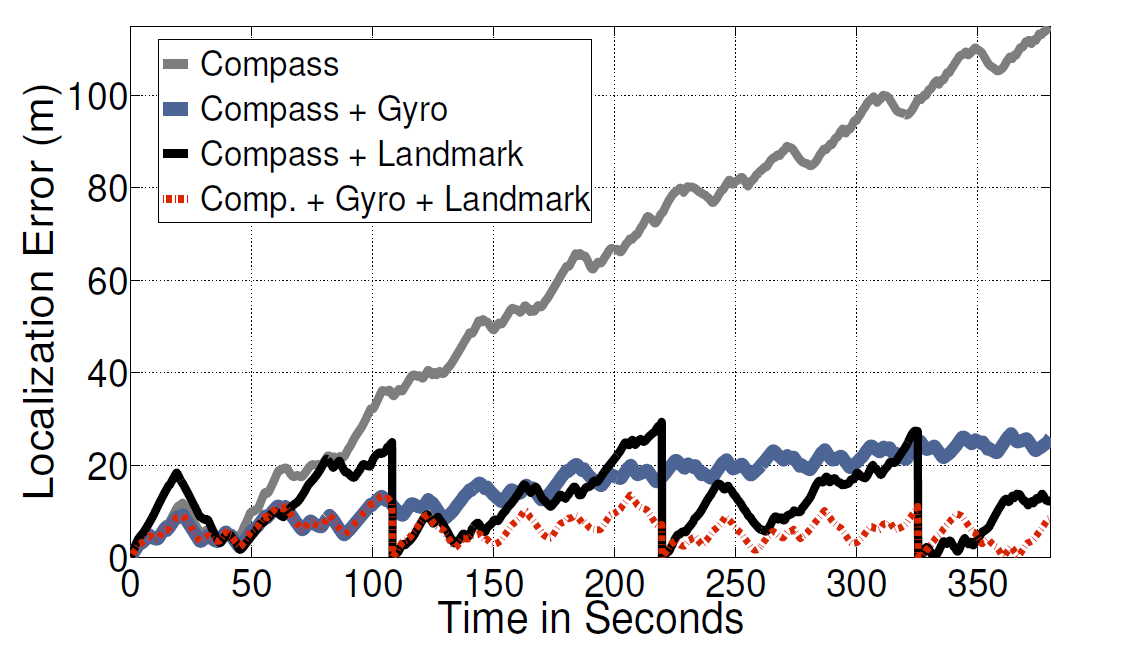
\includegraphics[width=0.7\textwidth]{dead.png}
                \end{figure}
                
                Such conventional methods had also been gradually improved upon to provide sub-metre levels of accuracy using by combining crowd-sourced data with probabilistic reasoning through a technique called `Horus' \citep{youssef2005horus}. The first step (and largest weakness) of the Horus system is the necessary collection of sample data from known locations to create an initial RSSI map. Data collected by users while positioning however now continues to feed back into the initial RSSI map as the team discovered that RSSI values from each AP are not independent with regards to time, so utilise an auto-correlation co-efficient ($\alpha$) to help isolate useful measurements. This co-efficient defines how similar readings in an area have been and augments the expected distribution of RSSI values for that area to allow for a much larger range if all observations have been very similar.
                
                Using this modified RSSI map, positioning is then broken down into multiple steps; first the user's `discrete' area must be determined as the most likely position, given all of the access points that are currently visible. From here, the system uses a function of both the $N$ most likely locations weighted according to their normalised probabilities and the average signal strengths over a small time window to smooth out the estimate. Finally, the system enables tracking of small-scale variations by noting that a user's location cannot change more than their speed would allow. By this notion, if the user appears to have moved more than a threshold amount more than their previous movement, a small-scale error is assumed so the system tries an estimation for all received AP RSSIs multiplied by $1$, $1+d$ and $1-d$ to find the highest likelihood and associated location.
                
                The final technique this paper will cover requiring no prior knowledge of the space, extra deployments or specific training set is Microsoft's `EZ' localisation system \citep{chintalapudi2010indoor}. The technique is centred around solving simultaneous equations to provide accurate estimates, similar to \citet{madigan2005bayesian} in looking for its parameters. However, the technique uses occasional measurements paired with GPS readings and clustering methods to reduce the search space to the most useful subset. 
                
                \begin{equation} \label{eq:EZdistance}
                    d_{ij} = 10^{\left(\frac{P_i - p_{ij}}{10\gamma_i}\right)}
                \end{equation}
                
                For each access point ($i$), the system attempts to solve for its X and Y location, transmit power ($P_i$) and path loss rate ($\gamma_i$). If the access point is visible from at least 5 locations where GPS lock was established ($j$), then these parameters can be uniquely identified through solving simultaneous equations (Equation \ref{eq:EZdistance}) for RSSI values ($p_{ij}$) from which the access point was seen and then using the gathered distances ($d_{ij}$) to trilaterate the 2D location of the AP. Solving even just one AP's parameters can cause a domino effect leading to more uniquely identifiable locations, solving more AP parameters and so on. Eventually though the dominoes stop and the system has to guess some parameters in order to continue and the search space can be incredibly large. To counter this, the EZ team created APSelect and LocSelect, two clustering algorithms that group access points and unknown locations into a single point if the RSSI values observed overlap \textasciitilde90\%, thereby reducing the number of unknown variables the system has to solve for, taking only a minimal accuracy loss in the process.
                
                The space is then searched through to find a set of parameters with the minimum error using a combination of genetic searching and gradient descent. To start with, a set of solutions with completely random parameters are selected and their fitness (mean absolute error) evaluated. From here, the top 10\% are kept unmodified, 10\% are randomly re-generated, 60\% are made as a combination of 2 random parents from the last generation (and enhancing them through gradient descent) and the last 20\% are made by taking a single random solution from the last generation and tweaking each parameter by a random amount (from an exponential distribution to allow for occasional large changes). This combination of solution generation techniques avoids the large number of potential global minima that come with so many parameters while exploring the state space relatively quickly.
                
                One final optimisation applied to their method is accommodation for relative gain. By identifying proximate locations in which measurements were taken by two different devices, their average RSSI values can be compared to find their approximate relative gain difference and normalise their RSSI values for use in simultaneous equations. With all of these techniques combined, EZ was able to perform comparably to RADAR on larger scale deployments without all of the pre-deployment effort and the search for optimal parameters could be re-run as the space being localised changes and more data comes in. The main disadvantages with this technique come simply from its marginally lower accuracy than techniques like Horus (Figure \ref{fig:EZHorusRADARComparison}) and the relatively high computational effort required to implement the technique and compute the results.
                
                \begin{figure}[h]
                    \label{fig:EZHorusRADARComparison}
                    \caption{Cumulative distribution function of distance error comparing Horus, RADAR and EZ IPS techniques \citep{chintalapudi2010indoor}.}
                    \centering
                        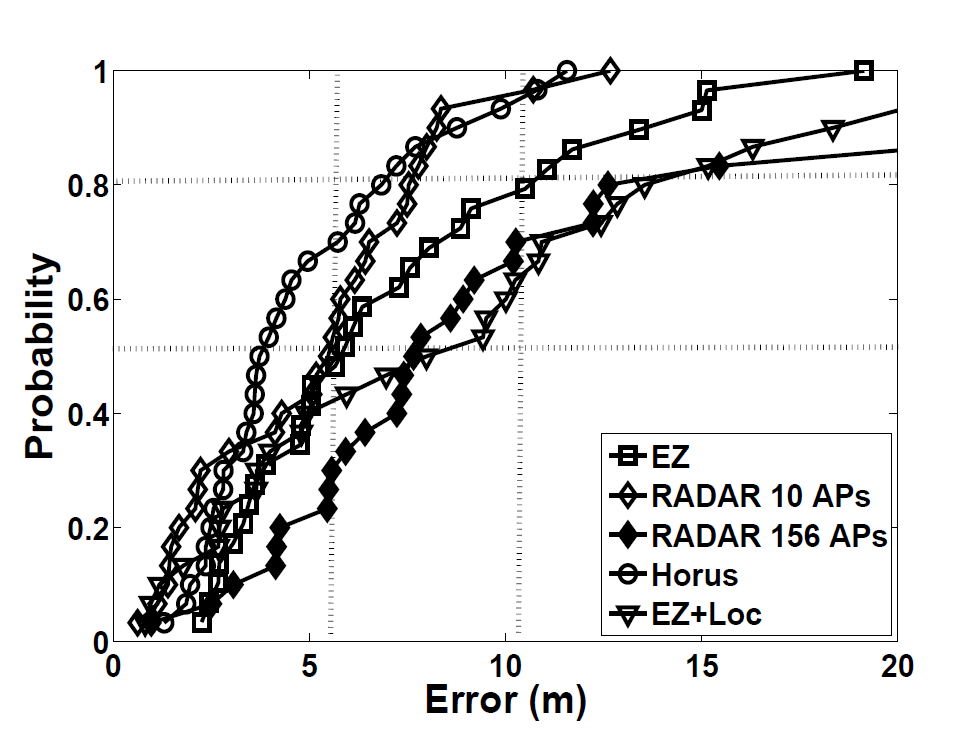
\includegraphics[width=0.7\textwidth]{EZHorusRADARComparison.png}
                \end{figure}
                
                Following the rapid development of IPS techniques \citet{torres2014ujiindoorloc} identified the need for a definitive data set to compare them through and created the UJIIndoorLoc database. The data set comprises of a large number of user-verified co-ordinates and their respective RSSI values to every WLAN access point being monitored. As these measurements were carried out by a number of users (integrating height as a differentiating factor) with a number of devices this provides great ecological validity to the data set while still delivering reliable measurements. The validation set was also generated without guide markers, ensuring that data different from the training set was provided. With such a comprehensive data set it is then easy to emulate limiting factors of any data gathering technique, such as noise or poor coverage, and due to high demand the team also provided a map of the locations \citep{UJIIndoorLocMap}. However, data points extraneous to the buildings in question would have been useful to provide a complete picture of a user's day both inside and outside of the buildings.
            
        \section{Automated Floor Plans}
        \label{sec:floorplans}
        
            Floor plans of a building are often key to enabling detailed location-based analysis by providing boundary information and special characteristics of the space, but may not be available prior to a system's deployment. It is easy to see how a special purpose robot might use a combination of dead-reckoning and obstacle sensors to map a space using an exhaustive search, but the cost of the equipment and the size of the area being surveyed could easily render the technique infeasible.
            
            Other techniques for building floor plans rely on gathering a small amount of pre-requisite data and building upon the constraints that it gives. A technique for determining layout on a small (single floor house) scale is described by \citet{lu2012smart} for use on ``Smart Homes''. Smart homes are buildings with a notion towards autonomous control, such as turning on the lights in the hallway before the user physically enters the space, detected through a collection of sensors placed about the home. Here, it is required to have motion detectors placed on both sides of every door (to determine room connectedness), a magnetometer (to determine door orientation) attached to these pairs of motion detectors and light level sensors on every window (facing inside and out, to determine orientation through sunrise / sunset). While this is a very high deployment cost through the level of user involvement, the deployed sensors are then anticipated to be in continuous use as part of the smart home itself.
            
            By monitoring the sensors to see which sets fire simultaneously, they can then be clustered into rooms to determine how many doors and windows each room has, and which rooms they are connected to. With the room's interconnectedness established, the technique then minimises the space of potential arrangements using a set of simple heuristics (i.e. windows tend to be on external walls and buildings have as few corners as possible). Despite all of these restrictions, the technique was only able to minimise the set to 2 or 3 potential layouts from which a user must select. As this technique was designed to prevent having a user draw their own plan it satisfies its purpose, but does not provide a detailed enough picture for fine-grain analysis or larger areas of observation.
            
            A more general approach to generating floor plans based on a set of constraints however comes from \citet{charman1994constraint}. This method mathematically defines a set of rooms based on their rotation, reference point and dimensions and attempts to fit them into a given space by connecting their corners. As the rooms are placed, a set of constraints are then evaluated and back-tracked upon where necessary (e.g. Bedroom \#1 must be to the right of Bathroom \#2). By exhaustively generating solutions, the system is able to find all possible layouts of rooms, given the pieces of data / constraints supplied. While successful at producing floor plans for traditional housing layouts, the method could fall short with modern architecture that often contains complex shapes (not squares) and unidentified empty spaces.
            
        \section{Summary}
        \label{sec:relsum}
        
	        This chapter has now broken down the work surrounding building analysis into the data gathering, data localisation and floor plan generation steps and provided a variety of techniques that are applicable at each stage. When gathering data from users it has been shown that techniques exist to reduce the load placed on users and their devices, potentially increasing the amount of data that would be gathered in a crowd-sourced technique through more opted-in users. While users are of the utmost importance when performing any crowd-based operations, this report focuses mainly on applications of the data once collected.
            
            When localising gathered data, a theme has emerged centring around the use of RSSI to estimate distances from access points. Despite its complex nature, the  widespread use and coverage of wireless networks combined with the success of simple models make it an attractive choice for IPS. Techniques explored here covered the fundamentals of modelling radio signal propagation, then demonstrated more advanced and novel techniques inferring unknown parameters through machine learning for ease of deployment and increased accuracy alike.
            
            Finally sets of constraints were identified for generating possible floor plans based on estimated dimensions. While restrictive in their application to walls in the four cardinal directions, this fits common traditional layouts of buildings and it is anticipated that more complex arrangements could be broken down into rectangular subspaces to build in. Through combinations of the described techniques this report will now explore ways in which a system might determine room usage from a set of simple crowd-sourced data.

    \chapter{Problem Analysis}
    \label{chap:problem}
    
        This chapter will explore the problem space involved with attaining the goals of the project. Primarily, this project is tasked with establishing a framework around which building analytic techniques might be developed or applied. This could include the development of any combination of the techniques covered in chapter \ref{chap:related} concerning crowd-sourcing the data, localising the data and modelling the space itself.
        
        Developing a complete system however would prove intangible for a project of this size as the system would require implementation across multiple platforms and likely multiple languages, carrying with it the interoperability complications to navigate and technical difficulties as opposed to research challenges. Furthermore spreading implementation time so thinly might also prevent any deeper evaluation as it would be hard to compare systems at such a high level. As such it would be wiser to focus on implementing a single component around which a system can be built.
        
        The first component to consider would be a modern crowd-sourcing tool-kit for specifying, gathering and collating some selection of data from sensors at minimal impact to the users. While implementing an application in Java using the techniques described in section \ref{sec:crowd} to enable gathering from a wide selection of Android devices would be beneficial to build from, it is known that a specific study into the factors surrounding crowd-sourcing data is running concurrently to this project \citep{IainBate}. Floor plan modelling using location data to feed a constraint solver such as that described by \citet{charman1994constraint} could also be an effective component. However, compiling such a complete set of data without implementing either of the previous components of the system would be very costly for such a small team, given the number of man hours it would take to exhaustively map out a significant area. Therefore, the most useful component to create as part of this project would be an Indoor Positioning System around which other techniques may be developed. As demonstrated by \citet{torres2014ujiindoorloc}, there exists a high demand for open implementations of such components and thanks to the existence of such sample data sets, the cost of testing and comparing such techniques are greatly reduced.
        
        As explored in section \ref{sec:ips}, there exist a multitude of techniques for localising users in an indoor space with varying degrees of accuracy. The goals of this project however, limit the range of applicable techniques as the model should be created from readily available sources of information. While this immediately rules out any infrastructured techniques as the installation of extra equipment severely limits the domain space that can be modelled, this project will also avoid those that require a large set of ground-truth, domain-wide test data as they are again limited in their application. With these restrictions in place the most interesting systems to study would be: RADAR \citep{bahl2000radar}, landmarked dead-reckoning \citep{wang2012no} and EZ \citep{chintalapudi2010indoor} from those evaluated in chapter \ref{chap:related}.
        
        RADAR provides one of the highest levels of accuracy of all reviewed techniques for relatively low localisation and model-building cost as it is all based around a pre-existing floor plan. Using this floor plan, the technique estimates the RSSI of every AP by using a simple formula modelling the signal's attenuation through walls and across space. In situations where detailed floor plans are already available, using this method could be the most efficient means for determining building usage metrics as the model building process is skipped entirely and user positions can be determined immediately. However, floor plans are not always complete, universally accessible nor consistent with flexible spaces such as exhibition centres. Because of this limitation in combination with the lack of information generated by skipping the modelling process, this technique is not useful for the project.
        
        Landmarked dead-reckoning appears to rectify most of these concerns as the technique requires no previous knowledge of the space (by dead-reckoning from a known point) and creates its map of landmarks that are potentially much less dependent on the flexible properties of the space (such as elevators and stairs). This enables the modelled space to change over time while preserving a relatively high level of relative location accuracy. Therein however lies the problem with using this technique to measure space utilisation as it can only detect relative movement as opposed to independent single-point localisation. This is not to say that the technique would be difficult to gather sample data as \citet{torres2015ujiindoorlocmag} provides the full complement of magnetometer, accelerometer and (in conjunction with future data to be provided by \citet{JoaquinEmail}) RSSI readings necessary to implement such a system. The worry is more about the load placed on prospective user's devices and how to gather meaningful results without the storage requirements becoming infeasible. As shown in the UJIIndoorLoc-Mag database, the \textasciitilde40,000 data points only correspond to \textasciitilde300 short relative motion traces so it is not unimaginable for the data sets to quickly get out of hand, especially if a user were to store multiple day's worth of data before a storage opportunity arises. Solutions to these problems could involve modifying the sampling frequency to reduce the load on the user's device and the amount of data held for analysis, but it is unknown as to how this would affect the accuracy of the model due to the precise nature of the landmarks. Also, the test data and initial research do not cover the prospect of spending a large period of time walking around the same space with no significant landmarks. In these cases, the behaviour would return to basic dead-reckoning and continually stack up inaccuracies, potentially invalidating the data. For these issues in combination, landmarked dead-reckoning does not significantly work in the project's favour.
        
        EZ however, implements a system requiring a very simple set of independent client-side measurements backed up by a server-side model that can adapt to a changing space as the set of observations grows, without human intervention (such as specifying a new floor-plan like RADAR). With this technique, RSSI measurements are provided along with GPS co-ordinates (where possible) to estimate the relative location and signal transmission properties of the access points being observed. This simplicity of the data required to build the model along with that of the model itself also makes it useful for research into building analytics as it reduces the effort required to crowd-source the data in the first place and reduces the complexity of any floor plan model wishing to reinterpret the EZ data.
        
        Assuming that the crowd-sourcing programme or test data input provides a reading of all RSSIs available (as already required by a wide range of infrastructureless indoor positioning systems) alongside the occasional GPS location, EZ will be able to provide a model for localising those without position data and any future measurements made. Furthermore, assuming that the floor plan modelling technique is also able to make use of positioning data, the output of running EZ on the original data set will still be useful regardless of the technique's ability to interpret the AP parameters to some degree. Combining these assumptions with a large set of sample data such as that provided by \citet{torres2014ujiindoorloc}, the EZ localisation component can then be developed independently of any crowd-sourcing or floor-plan modelling strategies that may follow.
        
        Unfortunately, \citeauthor{chintalapudi2010indoor}'s implementation of EZ is proprietary property of Microsoft and as such was not available for inclusion in this project. Re-implementing the system however provides an opportunity to evaluate the specification provided against a number of non-functional metrics as well as the modelling accuracy. For example, re-implementation and testing against a new data set may highlight a number of hidden assumptions and scenarios in which the model is flawed impacting directly on its applications for the real world and the ease of development for a more novice team. This project's implementation will also be aligned with a different set of goals, such as extensibility and flexibility (with regards to testing parameters and components) as opposed to raw throughput for a single space that a commercial solution might strive for.
 
	\chapter{Method}
    \label{chap:method}
	
		This chapter will cover the development of an indoor positioning system from which positioning data and Wireless AP models can be extracted for use as part of a general building model. The  model will follow the techniques as specified in the EZ localisation system \citep{chintalapudi2010indoor} with measurements from the UJIIndoorLoc data set for testing and evaluation purposes \citep{torres2014ujiindoorloc}. This chapter will also identify some weaknesses in the specification of EZ and propose the Heuristic-EZ localisation system to compensate.
		
		\section{System Specification}
        \label{sec:sysspec}
            
            Microsoft's proprietary implementation of EZ by \citeauthor{chintalapudi2010indoor} consisted of ``about 7000 lines of C\# and Python code'' encompassing all of the client-server communications, data gathering and off-line modelling /on-line localisation operations. By separating out the data processing elements of EZ from the rest of the system, this implementation of EZ can take advantage of languages with more powerful built-in mathematical functionality without worrying about handling sensors and external communications. As such this project will pursue an implementation in Matlab 2015b consuming a .CSV file of pre-gathered measurements and outputting two .CSV files containing all localised points and the AP parameters separately. This allows future efforts into crowd-sourcing to take advantage of techniques available to other languages while still piping data into this implementation of EZ. It will also allow floor plan modellers to be selective as to which types of data they wish to use to generate their models, again in their language and platform of choice.
            
            \begin{figure}[h]
            \label{fig:EZControl}
            \centering
            \resizebox {\textwidth} {!} {
            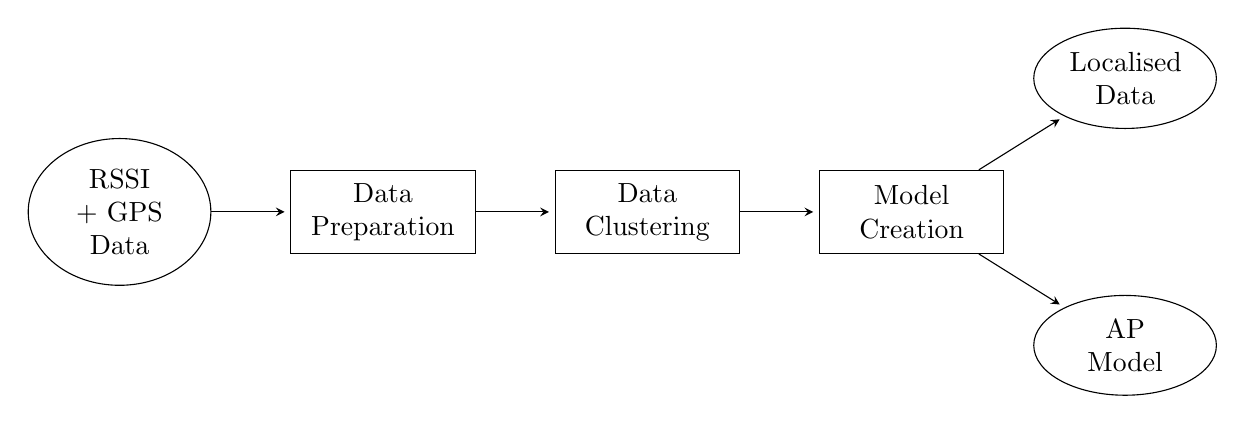
\begin{tikzpicture}[%
            ->,
            shorten >=2pt,
            >=stealth,
            node distance=1cm,
            process/.style={%
            	rectangle,
            	text width=6em,
            	minimum height=3em,
            	align=center,
            	draw
            },
            data/.style={%
            	ellipse,
            	text width=4em,
            	align=center,
            	minimum height=3em,
            	draw
            }
            ]
            \node[data] (1)                                 {RSSI + GPS Data};
            \node[process] (2) [right=of 1]                 {Data Preparation};
            \node[process] (3) [right=of 2] 				{Data Clustering};
            \node[process] (4) [right=of 3]                 {Model Creation};
            \node[data] (5) [above right=of 4]              {Localised Data};
            \node[data] (6) [below right=of 4]              {AP Model};
            
            \path (1) edge             node {} (2)
            (2) edge                   node {} (3)
            (3) edge                   node {} (4)
            (4) edge                   node {} (5)
            (4) edge                   node {} (6);
            \end{tikzpicture}
	        }
            \caption{EZ Control Flow}
	        \end{figure}
            
            EZ's specification then breaks the system down into a set of components, each of which is able to operate independently of the others or chained together for various effects. To this end, the project's implementation of EZ will take a pipe \& filter approach allowing each component to affect the data in turn before passing it on to the next (see Figure \ref{fig:EZControl}). These components will all operate without knowledge of the other's actions and upon the same data format, such that components may be changed for different versions or removed entirely without significantly impacting the program's flow.
            
            The creation of EZ's model is the first and only mandatory component specified, but also comes as the final piece of any system variant that might be created. Given a set of data this component will attempt to create a model based on the idea that with enough already localised measurements of RSSI from an AP, some basic parameters can be estimated about the object (giving the AP model data). Then if a measurement without GPS data can view enough parameterised APs, then its location can be trilaterated using simultaneous equations (this will be covered in detail in section \ref{sec:modelcreation}).
            
            However, as is also specified, the data can be effectively refined and reduced before it is passed to the model creator through preparation and selection of the most useful pieces of data. The most prominent piece described for preparing data is that of gain estimation as they appeared to find gain differences of up to \textasciitilde14dB which could significantly distort models generated using that data by making measurements taken at the same location on different devices appear very different by RSSI. To alleviate some of these problems, they propose the Relative Gain Estimation Algorithm (RGEA) which looks for small, consistent differences in RSSI measurements and creates a set of estimated differences in gain across devices. By solving these differences as a set of simultaneous equations, the gain values of each individual device can be estimated and used to correct the input data (covered in full in section \ref{sec:dataprep}).
            
            Finally covered is the selection of specific data points to use when modelling through the use of hierarchical clustering. This clustering algorithm aims to group data points of 90\% or greater similarity and then nominate a representative from each group to be passed to the model. The algorithm is run twice on the same data set, but once to select the most useful Access Points (APSelect) and once to select the most useful measurement locations (LocSelect) for different reasons. APSelect is run to reduce the number of APs modelled as the team observed up to ``160 APs across a single office floor'', potentially leading to an over-constrained model and excessive modelling time. LocSelect however, is necessary to prevent biases in the model where too many measurements from the same location may reduce accuracy in others.
            
            The ordering of these components is of course fixed as clustering data without correcting for gain could miss potential groupings and correcting the gain of already localised points would lead to inaccuracies. The components can however be avoided entirely (except for modelling) as \citeauthor{chintalapudi2010indoor} experimented with. This project will make comparisons of its implementation to their claims using their `\emph{LARGE}' data set as its size is more comparable to a single floor of a building in that of the work by \citet{torres2014ujiindoorloc}.
		
		\section{Data Preparation}
        \label{sec:dataprep}
        
            In order to compensate for artificial noise created by differences in gain across devices measuring RSSI at the same location, the RGEA estimates these differences and applies them to the data set. However, with only a subset of the data having a known location, the RGEA has to use RSSI to guess at `proximate' locations. The specification states that measurements are deemed proximate if the average difference between RSSIs is less than 3dB. For each pair of devices ($k_1,k_2$), these pairs of measurements are then gathered into a set $M^{k_1k_2}$ and compared to get the average difference (Equation \ref{eq:avggaindiff}). This relative gain is then plugged into equation \ref{eq:stddevgain} to calculate the standard deviation of that relative gain from the difference in all comparable measurements.
            
            \begin{equation}
            \label{eq:avggaindiff}
                \Delta G^{k_1k_2}=\dfrac{1}{|M^{k_1k_2}|} \sum_{(p_1,p_2)\in M^{k_1k_2}} (p_1 - p_2)
            \end{equation}
            
            \begin{equation}
            \label{eq:stddevgain}
                \sigma(\Delta G^{k_1k_2})=\dfrac{1}{|M^{k_1k_2}|} \sqrt{\sum_{(p_1,p_2)\in M^{k_1k_2}} (p_1 - p_2 - \Delta G^{k_1k_2})^2}
            \end{equation}
            
            Because these relative gains are transitive (i.e. $\Delta G^{k_1k_3} = \Delta G^{k_1k_2} + \Delta G^{k_2k_3}$), any pairs of devices with proximate locations can then be chained together with other device pairs to create a system of simultaneous equations. Finally a random device as part of this system is selected and chosen to have some value of gain and so the system can be solved. As this is an estimate however, the equations are weighted according to their standard deviation or in effect their likelihood of being accurate.
           
            Implementing this short specification however, leads to incorrect results. The main discrepancy is the selection of RSSI readings to include when comparing a pair of measurements. For completeness, the UJIIndoorLoc data set includes every invisible AP as a measurement of 100dB to mark it as an invalid measurement. If all readings (including invisible markers) are compared for a pair of measurements, then in spaces where only a small proportion of APs are visible at any given location, all locations will be deemed proximate as all invisible APs register a difference of $0$. The opposite however also causes problems, if only points visible at both locations are compared, then being equidistant from a single AP could cause the whole measurement to be deemed proximate (see Figure \ref{fig:overlap}). The solution is to compare all readings visible in either measurement, such if the measurement were to be localised using the set of points, they would be equal. However, including readings in this manner with the UJIIndoorLoc positive invisibility indicator causes any single difference in AP visibility, no matter how weak (i.e. -99dB), to be marked as not proximate in error. The simple fix was to change all 100dB readings to -100dB.
            
            \begin{figure}[h]
            	\centering
            	\begin{minipage}{0.45\textwidth}
            		\centering
                    \label{fig:overlap}
            		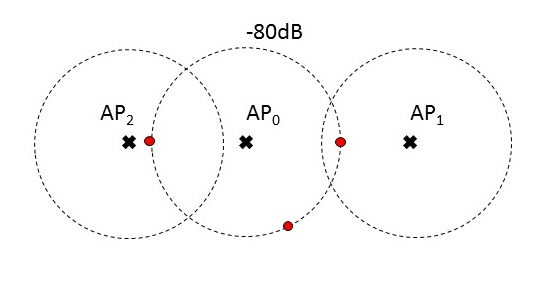
\includegraphics[width=\textwidth]{single_overlap.jpg}
            		\caption{All locations demonstrated would be marked as proximate with $0$dB gain when only using APs visible at both locations.}
            	\end{minipage}\hfill
            	\begin{minipage}{0.45\textwidth}
            		\centering
                    \label{fig:wall}
            		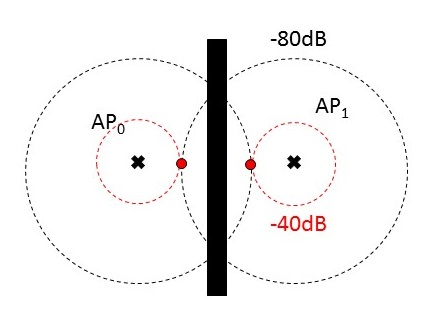
\includegraphics[width=1\textwidth]{wall.jpg}
            		\caption{Across wall case mistakenly marked as proximate with $0$dB gain.}
            	\end{minipage}
            \end{figure}
            
            With the specification implementation producing feasible results, it was at this point that the technique was to be validated against some known values. With no provided gain values for the devices in use by UJIIndoorLoc however, it was necessary to attempt to calculate them separately. To this end another relative gain estimator was created using the ground truth location values to specify exactly which pairs of measurements were proximate. The first major change was the addition of a general location translator to the data preparation phase as measurements were gathered within a few hundred metres of each other, but the latitude values started at \textasciitilde4,865,000m. The other major difference was a factor of speed. As the location comparison only needed to compare the difference between latitude and longitude as opposed to the average difference of up to 520 APs, the ground truth calculator performed over 2 orders of magnitude faster!
            
            Through experimentation and comparing the RGEA's output with the newly calculated values, several other faults of the implementation came to light. The first was that when calculating the average difference between measurements for inclusion in the set $M^{k_1k_2}$, it was meant to be the average \emph{absolute} difference being less than 3dB. Errors in light of this fault arose with measurements where readings balanced out with positive and negative differences (such as being opposite sides of a wall). For example the average difference of (-20dB, 20dB) for 2 APs is $0$dB, causing the points to be falsely identified as proximate with no relative gain (see Figure 4.3).
            
            Despite removing the majority of the falsely proximate points through this fault, the technique would still produce a very small number proximate points for those that should have none in common due to random fluctuations in the RSSI. Because of the transitive nature of the relative gain, this lead the algorithm to attempt to include erroneous relationships in its system of simultaneous equations, rendering them either unsatisfiable or wildly overestimating the gain applied to certain devices. As such the simplest solution was to impose a minimum number of proximate points for a relative gain to be of great enough significance to consider in the system.
            
            Given the computational and general modelling complexity of EZ's RGEA, it was theorised that there could be some simpler proximity metric with computation times more similar to those of the ground truth estimator. This lead to the creation of the first simplified component of this study: 'Heuristic RGEA'. Rather than essentially re-calculating the potential relative gain for every point, this technique compares the AP visibility of the strongest RSSIs at each location. Simply put, for each pair of measurements, if both samples have at least a certain number of RSSIs above some strength threshold, the locations can be deemed proximate if the strongest set is similar \emph{by AP ID alone}.
            
            This metric should prove effective because of the abundance of APs shown in both \citeauthor{chintalapudi2010indoor}'s study \citep{chintalapudi2010indoor} and the UJIIndoorLoc data set \citep{torres2014ujiindoorloc} creating an AP fingerprint for most locations. Initial tests however did highlight that the ordering by strength within these fingerprint sets is almost never identical due to random fluctuations in RSSI, leading to an extremely pessimistic judgement of proximity, as such the final implementation only specifies a minimum overlap between the two. With a number of parameters available to tune that may greatly affect the outcome of relative gain estimation (including the average difference threshold for EZ's RGEA and the size of the strongest set to compare in Heuristic RGEA), both techniques will be experimented with in section \ref{sec:rgeaeval}.
		
		\section{Hierarchical Clustering}
        \label{sec:datacluster}
        
	        In EZ, hierarchical clustering is used to effectively reduce the set of data fed into the modelling process both for speed and to reduce bias. The technique is used both as part of processes called APSelect to determine which APs are to be modelled by the system and LocSelect to choose the subset of all measurements around which to model them. To prepare the data for clustering, each measurement is normalised across the range ($0 \rightarrow 1$) for RSSIs ($-100 \rightarrow 0$) where any unseen APs have their RSSI set to -100dB. Clusters are then grouped if the average absolute difference between every pair of measurements across clusters is less than $0.1$ (>90\% similarity). Finally the point elected to represent each cluster is that which is most constrained (can see the highest number of GPS localised measurements in APSelect or just a binary indicator of being GPS localised in LocSelect) and the most similar to the rest of the cluster in the case of ties.
	        
	        Interestingly, \citet{chintalapudi2010indoor} only discuss the effect of removing fringe-case data points for speed improvements with regards to the modelling stage. However, as is especially notable with the UJIIndoorLoc data set, there may exist more significant measurements or (less commonly) APs in very close proximity which should also be clustered into a single representative point. This has the effect of reducing bias towards these locations by removing the error incurred from their use in the modelling stage.
	        
	        While simple and theoretically sound, this naive implementation of clustering doesn't take into account the potentially sparse nature of the input data with regards to AP visibility. When run for APSelect over the UJIIndoorLoc data set, more than 10,000,000 full data set comparisons were required (taking hours to complete alone without modelling) and LocSelect over a thousand point data set was rendered computationally intractable. The results also suffered a similar problem to that of the RGEA where given enough measurements / APs, `invisible' RSSIs outweigh those of any significance so a much greater amount of clustering occurs than should be necessary.
	        
	        In an attempt to minimise these issues, MATLAB's sparse matrices can be employed if making full comparisons per point (to little effect) but to get a less aggressive clustering, techniques explored during the creation of the RGEA can be employed. The first of these is to use a much simpler indicator as to whether the points might be similar before running the calculation, the most obvious of which is simply the set of non-zero measurements. If the set overlaps enough (differing in size dependent on the number of non-zero measurements per point) then a comparison over the union of both of these sets should be run.
	        
	        This idea can then be extended to only consider the high strength measurements from each point as they are the least prone to noise and likely to be reliable for modelling. By only considering measurements above a threshold this comparator also creates a 'zero' category where measurements for the point were not considered reliable enough and skipped entirely, providing a significant speed increase by immediately removing points from clustering. Removing these fringe-case measurements however, may also impact on a location's instant recognisability. For example, if an AP belongs to a neighbouring building and is only visible in a very small area on the edge of the building being modelled, then seeing that AP could immediately narrow down the location of the data point (see Figure \ref{fig:fringe}). The impact of these various attempts at data set reduction will be evaluated in section \ref{sec:modeleval}.
		
		\section{Model Creation}
        \label{sec:modelcreation}
        
            This final section will cover the main modelling component of the system, taking in processed data from the previous components and deriving a model of the AP layout and signal transmission properties surrounding them. Interesting challenges of dealing with real-world scenarios (discovered through rudimentary verification testing) will be explored and the process of using the model to localise measurements will be described.
        
            \subsection{Off-line Learning}
            
                The off-line learning phase of this component is concerned with translating the input data into a simple model of all APs through solving systems of simultaneous equations. For each AP, the system has to choose a distance to each observation $d_{ij}$ (and by extension a latitude and longitude location), transmission power $P_i$ (starting strength) and path loss rate $\gamma_i$ (signal strength fall-off curve). If the model were perfect, these 4 parameters could be uniquely determined (single global minimum error) from just 5 observations of the AP from known locations by minimising the RSSI error produced by equation \ref{eq:modelerror}.
                
                \begin{equation}
                \label{eq:modelerror}
                    error_i = \frac{1}{N}\sum_{ij}|p_{ij} - P_i + 10*\gamma_i\log{d_{ij}}|
                \end{equation}
                
                This model however lacks the ability to show sudden drops in signal strength and instead will choose to model the AP as closer to its observations with a higher path loss rate (as demonstrated in their study \citep{chintalapudi2010indoor}). As the solution space per AP is so large, this inaccuracy coupled with the potential random fluctuations in RSSI can lead to a large number of plausible parameters. \citeauthor{chintalapudi2010indoor}'s implementation employed a complex genetic algorithm considering many solutions per iteration in order to explore the space quickly. For drastically reduced implementation and modelling time however, this project opts to use a constrained version of Matlab's simulated annealing.
                
                The search space is constructed with reasonable allowances for signal transmission parameters (according to \citet{chintalapudi2010indoor}) and a bounded space around the included observations. Within that, the starting point is set as the average location of the included observations as might be common in a central AP deployment. This starting point is of lesser significance however, as simulated annealing provides a non-deterministic element to the gradient descent unlike other function minimisers, leading to less reliance on a good starting point. The main constraint on the simulated annealer is actually over the sufficiency of its output; given its semi-random, single solution nature, it is possible for the annealer to miss all plausible solutions and output a model-skewing set of bad AP parameters. As such, if the annealer's solution re-localises the modelling data to a median error of more than 10m, it is re-run up to a maximum of 10 times at which point the AP is deemed unsatisfiable and removed from the model.
                
                After attempting to model several APs it became apparent that a much larger proportion was being deemed unsatisfiable than initially anticipated, despite having a significant number of observations. The problem with these APs was that they appeared to be located on other floors of the same building. While theoretically plausible given enough data and time to model the extra dimension for AP placement, this project aimed to remain in the more proven 2D subspace (as demonstrated through the review of work in section \ref{sec:ips}). As such, the set of weak measurements coming through the floor to a small area was being interpreted as a large distance from the AP, but then being modelled laterally rather than vertically (see Figure 4.5).
                
                \begin{figure}[h]
                	\centering
                	\begin{minipage}{0.45\textwidth}
                		\centering
                        \label{fig:fringe}
                		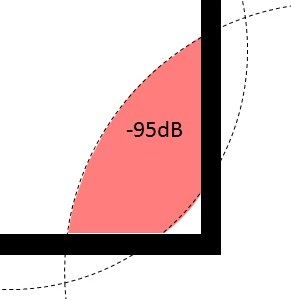
\includegraphics[width=0.7\textwidth]{fringe.jpg}
                		\caption{Red area marking the localisable fringe-case zone of a building.}
                	\end{minipage}\hfill
                	\begin{minipage}{0.45\textwidth}
                		\centering
                        \label{fig:vertical}
                		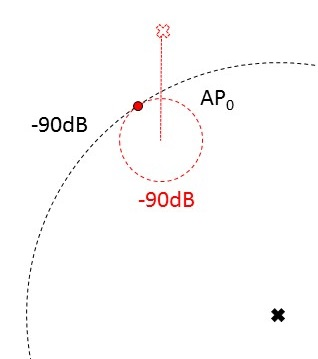
\includegraphics[width=0.7\textwidth]{vertical.jpg}
                		\caption{Visual representation of the difference between modelling an AP vertically (red) and laterally (black).}
                	\end{minipage}
                \end{figure}
                
                While potentially very useful towards localising to a very specific area of a floor, such a small area of coverage would be impossible to model without greatly expanding the search space for every AP. Given that these signals were also passing through concrete, electrical cables and various pipes to be received, the signals might also be particularly prone to interference and as such inaccurate beyond identifying the general area that the measurement was taken. Without ground truth data about the APs that would allow for model comparison and preparatory pruning of those less directly useful (though more thorough data covering alternative spaces are anticipated through communication with \citet{JoaquinEmail}), a thresholding heuristic was devised in place.
                
                Thresholding simply prunes all RSSIs below a certain level for both modelling and localisation purposes in an attempt to split the 3D space into an independent set of 2D subspaces. Pruning in this manner will significantly reduce the localisable area surrounding an AP, but as a consequence it should also increase the overall reliability of the set of measurements used by reducing the signal-to-noise ratio. However, it is also necessary to prune the same measurements for localisation so as not to incorrectly extrapolate the path loss rate at longer ranges, further reducing the localisability of most points.
                
                This technique could also be applied as an alternative to the hierarchical clustering component by simply requiring APs and measurements to have a minimum number of high strength RSSIs. While it is anticipated that this would not cluster extremely similar, high-strength points as discussed in section \ref{sec:datacluster}, it should be able to identify weak, fringe-case points in just linear time. By using some form of parameter optimisation (i.e. simulated annealing) over a combination of these thresholding techniques, it was anticipated that a strong separation across floors could be established without over-restricting the coverage of each AP. This level of complexity however would run contrary to the initial time savings made and potentially over-fit to each set of data. As such, experiments will be performed in section \ref{sec:modeleval} to determine a general purpose set of parameters that increase localisation accuracy without drastically restricting coverage.
                
                The final parts of the modelling process deal with insufficiencies in the input data: AP propagation and the ERSGA. AP propagation tackles the fact that GPS or other positional data is often not available throughout buildings and as such not all modelling data will have pre-associated positions. The solution is to iteratively generate AP parameters based on the localised data points and then localise new data points using the parametrised APs. The EZ Random Solution Generation Algorithm (ERSGA) however attempts to create AP parameters where there are simply not enough points observing it. While novel and potentially effective at producing models for areas poorly covered by the data with a full genetic algorithm, for this project it would add needless complexity (both for implementation and at run-time) to increase accuracy in the fringe-case areas that most components so far have sought to eliminate. As such the ERSGA is not implemented in this project and the assumption is made that a crowd-sourced data set should be suitably thorough and cover all useful locations.
            
            \subsection{On-line Localisation}
            
	            Localisation of new data points using this model is a much simpler process, simply plugging in the observed RSSIs for all modelled APs into equation \ref{eq:EZdistance} to obtain an estimation of distance. As these APs also have a fixed location, so long as the data point can see at least 3 modelled APs the location of the data point can be found through trilateration. Even with the inaccuracies produced by random fluctuations in RSSIs, there should exist a single global minimum for distance error when solving for the latitude / longitude location. This combined with the fact that the solution only requires the two location parameters, it is just as effective and much faster to use a least-squared error simultaneous equation solver rather than including the overheads associated with a simulated annealer.
	            
	            It is unexplored at this point however as to how the selection of modelled APs from which the point is localised might affect accuracy. For example, during the AP propagation phase of modelling, a data point is localised as soon as enough of its observed APs are parametrised but it might be more effective to restrict localisation to more reliable measurements. To this end, using the thresholding technique from the modelling phase will impose this restriction, but the maximal set heuristic from other components can also be applied in a similar manner. By restricting localisation to over the strongest (and most likely reliable) RSSIs, the system might be able to achieve higher localisation accuracy by avoiding weaker conflicting measurements where possible without removing coverage outright that might occur from thresholding. As such the various combinations of restrictions, component types and localisation methods will be evaluated for accuracy in section \ref{sec:modeleval}.
        
	\chapter{Evaluation}
    \label{chap:eval}
    
	    \section{Relative Gain Estimation}
	    \label{sec:rgeaeval}
	    
		    \subsection{Proximity Determination}
		    
		    \subsection{Gain Estimation}
	    
	    \section{Modelling Accuracy}
	    \label{sec:modeleval}
	    
		    \subsection{Component Effectiveness}
		    
		    \subsection{Restricted Modelling Performance}
	
		\textcolor{red}{Save actual quantifiable results for this section! Evaluate against requirements / massive discrepancies in method.}
		\begin{itemize}
			\item Parameter experimentation
			\item Use PlotFloor to show difference between models with various pieces of the system included / excluded and parameters tweaked
			\item Evaluate with noisy and partially localised data (explain how this is unrealistic though because we cannot tell what data around the edge would truly be localised, so we just remove the location from random points)
            \item Independent vs. estimating every APs parameters at once?
			\item Note EZ specifically says it works best with a large amount of data distributed across the whole area whereas UJIIndoorLoc provides with lots of measurements from the same locations. Will be interesting to see accuracy when used on an actual crowd-sourced deployment / samples collected from randomly generated locations.
			\item Show validation as well as evaluation of new model - explain increasing threshold will remove potentially useful boundary cases, but remove a large amount of useless noisy data.
			\item Validation should mainly be shown through qualitative justification and explanation, but can be done over a large number of tests (multiple runs on multiple floors and buildings) in the absence of mathematical proof.
			\item Test same parameters across other data sets (library and computer lab) for consistent levels of accuracy
            \item \textcolor{blue}{RGEA evaluations: RGEA pessimistic, Heuristic optimistic. On further inspection though, a number of those identified as false positives had differences of 2dB between the same three APs identified as strongest, but the measurements were taken a whole floor and over 10m laterally apart! Evaluation run over how effectively the points were determined as proximate as then you can compare only APs visible to both locations to avoid clipping of RSSIs below the detection threshold. Good gain estimation though despite false positives (at least on single floors)}
            \item Do a run where simulated annealing runs 1000 times or until it finds an error of < 3m. Does that significantly increase the model's accuracy?
            \item \textcolor{red}{HOW TO DISPLAY DATA}
		\end{itemize}
		
		\textcolor{green}{\emph{\[GOOD PIECES WITHIN\]}Testing should show validation as well as evaluation of the new model. Validation could explain how increasing threshold level will remove APs from other floors, but also potentially remove small overlaps from nearby buildings (i.e. if an AP is visible only in a small area near the edge of the building, seeing that AP means the location must me in that space). A similar effect could potentially be observed across floors (i.e. the AP only being visible if the location is directly below it), but this would require a much wider domain for parameters, such as extremely low transmission powers or extremely high path loss rates. However, use of these extremes, could be identified and used to help place the AP on another floor with some defined loss across floors like the WAF used in RADAR.}
	
	\chapter{Conclusion}
    \label{chap:conclusion}
    
	    \begin{itemize}
	    	\item Crowd-sourced building analytics is a large field requiring multiple components to operate, but each piece is independent enough to allow for development by small teams
	    	\item Components are underspecified from model given by paper
	    	\item Effectiveness of initial EZ model does not stretch to larger / more complex areas under modelling
	    	\item Heuristic components improve on speed and accuracy of EZ's IPS
	    	\item Framework now prepared for future work on crowd-sourced building analytics
	    \end{itemize}
	    
	    Further Work:
	    \begin{itemize}
	    	\item Validation against a real-world crowd sourced data set necessary
	    	\item Make use of absence of signal / fringe cases
	    	\item Compare AP model info to ground truth AP parameters
	    	\item Model 3D space through either inclusion of 3rd dimension or model 3D as a set of 2D layers
	    	\item Horus methodology - use strongest measurements to define fingerprinted area, then use weaker measurements to refine position
	    \end{itemize}
    
    \textcolor{red}{\emph{MAKE SURE YOU CHECK YOUR REFERENCES ARE CORRECT!}}
        
    \bibliography{report.bib}
	
\end{document}
